\begin{figure}[ht!]
    \centering
    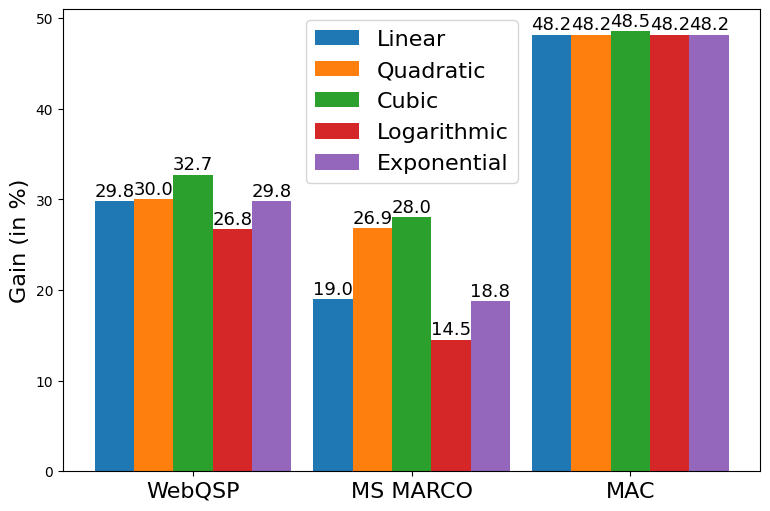
\includegraphics[width=\linewidth]{image/ablation_study.png}
    \caption{Gains across different penalty functions. \textit{Cubic} penalty obtains the best gains across three datasets.}
    \label{fig:ablation_study}
    % \vspace{-1em}
\end{figure}

We now present an ablation study to evaluate the impact of different formulas for the penalty function $F(\rr)$ on \rap (Equation \ref{eq:rap}). We consider five options including \textit{Linear}, \textit{Quadratic}, \textit{Cubic}, \textit{Logarithmic}, and \textit{Exponential} where the penalty are $1-\rr$, $(1-\rr)^2$, $(1-\rr)^3$, $\text{log}_{2}(2-\rr)$, and $e^{-\rr}$, respectively. 
%
We compare the \textit{Gain} achieved with each repetition penalty formula. For a model, \textit{Gain} is defined as the difference between the reduction in repetition and the performance drop when tuning RPP using original performance versus RAP. It reflects how much repetition decreases (i.e., gain) relative to the performance loss when tuning RPP with RAP. The higher \textit{Gain}, the better. 
%
Figure~\ref{fig:ablation_study} shows the \textit{Gain} scores for each formula across the three datasets. The \textit{Gain} for a dataset is calculated by averaging the \textit{Gain} values from all models and prompting strategies. 
% The results show that the \textit{Cubic} penalty consistently achieves the highest gain across all datasets (32.7\% for WebQSP, 28.0\% for MS MARCO, and 48.5\% for MAC), indicating it offers the best balance between reducing repetition and maintaining performance. Notably, all penalty formulas perform similarly well on MAC, with gains around 48\%, suggesting the choice of penalty is less critical for tasks where performance is less sensitive to repetition reduction like MAC. These findings support using the \textit{Cubic} penalty for the RAP metric as it provides a strong balance across varied datasets and tasks.
The results show that the \textit{Cubic} penalty consistently achieves the highest gains across all datasets (32.7\% for WebQSP, 28.0\% for MS MARCO, and 48.5\% for MAC), offering the best balance between reducing repetition and maintaining performance. These findings recommend the \textit{Cubic} penalty for the RAP metric, as it performs well across diverse datasets and tasks.

% The results show that \textit{Cubic} penalty consistently achieves the highest gain across all three datasets (32.7\% for WebQSP, 28.0\% for MS MARCO, and 48.5\% for MAC). This indicates that the cubic function provides the most optimal balance between reducing repetition and preserving model performance.
% Interestingly, all penalty functions perform similarly well on MAC, with gains hovering around 48\%. This suggests that the choice of penalty function may be less critical for tasks or datasets where performance is less sensitive to repetition such as MAC. 
% These findings support our choice of the \textit{cubic} penalty function for the RAP metric, as it provides a robust balance between repetition reduction and performance preservation across diverse datasets and tasks.




% The results highlight several key findings:

% \noindent \textbf{Superiority of Cubic Penalty:} The \textit{cubic} penalty function consistently achieves the highest gain across all three datasets (32.74\% for WebQSP, 28.03\% for MS MARCO, and 48.54\% for MAC). This indicates that the cubic function provides the most optimal balance between reducing repetition and preserving model performance.

% \noindent \textbf{Consistency Across MAC Dataset:} Interestingly, all penalty functions perform similarly well on the MAC dataset, with gains hovering around 48\%. This suggests that the choice of penalty function may be less critical for tasks or datasets where performance is less sensitive to repetition, such as in the MAC dataset.

% \noindent \textbf{Variation Across Datasets:} The \textit{logarithmic} and \textit{exponential} penalty functions exhibit varied performance across datasets. While they perform relatively well on the MAC dataset, they lag behind the polynomial functions (linear, quadratic, and cubic) on both WebQSP and MS MARCO, indicating that the effectiveness of these functions may be task- or dataset-dependent.

% These findings support our choice of the \textit{cubic} penalty function for the RAP metric, as it provides a robust balance between repetition reduction and performance preservation across diverse datasets and tasks.




% The \textit{Gain} is defined as the difference of repetition ratio deduction and performance deduction, i.e., how much repetition drop versus how much performance drops, the large \textit{Gain}, the better. 



% \rap integrates \rr into the overall model performance by applying a penalty function to repetition in the generated content, as defined in Equation~\ref{eq:rap_generic}.

% \begin{equation}
%     \text{RAP} = P \times f(x)
%     \label{eq:rap_generic}
% \end{equation}

% Where $P$ is the performance metric (e.g., F1 score), $f(x)$ is a penalty function, and $x = 1 - \text{RR}$.

% We evaluated the following penalty functions:

% \begin{align}
%     f_{\text{linear, quadratic, cubic}}(x) &= x^n \quad \text{where} \, n \in \{1, 2, 3\} \\
%     f_{\text{logarithmic}}(x) &= \log_2(1 + x) \\
%     f_{\text{exponential}}(x) &= e^{x - 1}
% \end{align}

% We define the \textit{gain} as:

% \begin{equation}
%     \text{Gain} = \frac{\text{RR}_{\text{original}} - \text{RR}_{\text{RAP}}}{\text{RR}_{\text{original}}} - \frac{P_{\text{original}} - P_{\text{RAP}}}{P_{\text{original}}}
% \end{equation}

% Where $\text{RR}_{\text{original}}$ and $P_{\text{original}}$ are the repetition ratio and performance at the best performance-tuned RPP, while $\text{RR}_{\text{RAP}}$ and $P_{\text{RAP}}$ are the corresponding values at the best RAP-tuned RPP.

% Figure~\ref{fig:ablation_study} presents the results of this ablation study, showing the gains achieved across three datasets—WebQSP, MS MARCO, and MAC—for each penalty function. The goal was to maximize the gain, i.e., to achieve the highest reduction in repetition with minimal performance degradation.

% \begin{figure}[ht]
%     \centering
%     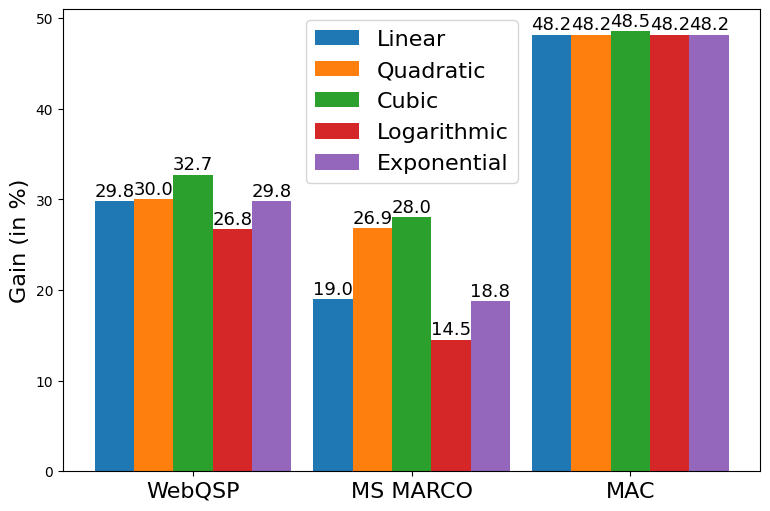
\includegraphics[width=\linewidth]{image/ablation_study.png}
%     \caption{Gains across different penalty functions on three datasets (WebQSP, MS MARCO, and MAC). The evaluated penalty functions include \textit{linear}, \textit{quadratic}, \textit{cubic}, \textit{logarithmic}, and \textit{exponential}.}
%     \label{fig:ablation_study}
% \end{figure}

% The results highlight several key findings:

% \noindent \textbf{Superiority of Cubic Penalty:} The \textit{cubic} penalty function consistently achieves the highest gain across all three datasets (32.74\% for WebQSP, 28.03\% for MS MARCO, and 48.54\% for MAC). This indicates that the cubic function provides the most optimal balance between reducing repetition and preserving model performance.

% \noindent \textbf{Consistency Across MAC Dataset:} Interestingly, all penalty functions perform similarly well on the MAC dataset, with gains hovering around 48\%. This suggests that the choice of penalty function may be less critical for tasks or datasets where performance is less sensitive to repetition, such as in the MAC dataset.

% \noindent \textbf{Variation Across Datasets:} The \textit{logarithmic} and \textit{exponential} penalty functions exhibit varied performance across datasets. While they perform relatively well on the MAC dataset, they lag behind the polynomial functions (linear, quadratic, and cubic) on both WebQSP and MS MARCO, indicating that the effectiveness of these functions may be task- or dataset-dependent.

% These findings support our choice of the \textit{cubic} penalty function for the RAP metric, as it provides a robust balance between repetition reduction and performance preservation across diverse datasets and tasks.